% To je predloga za poročila o domačih nalogah pri predmetih, katerih
% nosilec je Tomaž Curk. Avtor predloge je Blaž Zupan.
%
% Seveda lahko tudi dodaš kakšen nov, zanimiv in uporaben element,
% ki ga v tej predlogi (še) ni. Več o LaTeX-u izveš na
% spletu, na primer na http://tobi.oetiker.ch/lshort/lshort.pdf.
%
% To predlogo lahko spremeniš v PDF dokument s pomočjo programa
% pdflatex, ki je del standardne instalacije LaTeX programov.

\documentclass[a4paper,11pt]{article}
\usepackage{a4wide}
\usepackage{fullpage}
\usepackage[utf8x]{inputenc}
\usepackage[slovene]{babel}
\selectlanguage{slovene}
\usepackage[toc,page]{appendix}
\usepackage[pdftex]{graphicx} % za slike
\usepackage{setspace}
\usepackage{color}
\definecolor{light-gray}{gray}{0.95}
\usepackage{listings} % za vključevanje kode
\usepackage{hyperref}
\renewcommand{\baselinestretch}{1.2} % za boljšo berljivost večji razmak
\renewcommand{\appendixpagename}{Priloge}
\usepackage{amssymb}
\usepackage{amsmath}

\lstset{ % nastavitve za izpis kode, sem lahko tudi kaj dodaš/spremeniš
language=Python,
basicstyle=\footnotesize,
basicstyle=\ttfamily\footnotesize\setstretch{1},
backgroundcolor=\color{light-gray},
}

\title{Nadzorovano modeliranje}
\author{Amon Stopinšek (63150273)}
\date{\today}

\begin{document}

\maketitle

\section{Uvod}
% V tem razdelku, ki naj bo kratek in naj obsega en odstavek z do 150
% besed, na kratko opišeš, kaj je bil cilj naloge.

V nalogi smo uporabili enostavne metode za napovedovanje. Glavni cilj naloge
je bila napoved ocen filmov posameznega uporabnika na podlagi ostalih uporabnikov.
Problem smo najprej rešili s pomočjo regresije, kjer smo napovedovali dejanske
vrednosti. Nato smo se problema lotili še s klasifikacijo, kjer smo ocene filmov
razdelili v dva razreda in za danega uporabnika napovedali v kateri razred bi
uvrstil posamezni film.

\section{Podatki}

% Če je naloga zasnovana tako, da vključuje analizo izbranih podatkov, v
% tem razdelku opišeš, kakšni so ti podatki in navedeš nekaj osnovnih
% statističnih lastnosti teh podatkov. Slednje vključujejo velikost
% podatkov (na primer število primerov, število in vrsto atributov), delež
% manjkajočih podatkov, opis in porazdelitev vrednosti ciljnih
% spremenljivk, in podobno. Če si podatke pridobil sam, tu opišeš, na
% kakšen način, kje in kako.

Pri nalogi sem uporabili podatkovno zbirko
\href{https://grouplens.org/datasets/movielens/}{Movie Lens}.

\section{Metode}

% Tu opišeš, na kakšen način si rešil nalogo (tehnike in metode, ki si
% jih uporabil). Lahko vključiš tudi zanimiv del programske kode, ki
% si jo morda pri tem razvil ali pa v poročilo dodatno vključiš sliko,
% kot je na primer slika~\ref{slika1}. Vse slike in tabele, ki jih
% vključiš v poročilo, morajo biti navedene v besedilu oziroma se moraš
% na njih sklicati.
%
% \begin{figure}[htbp]
% \begin{center}
% 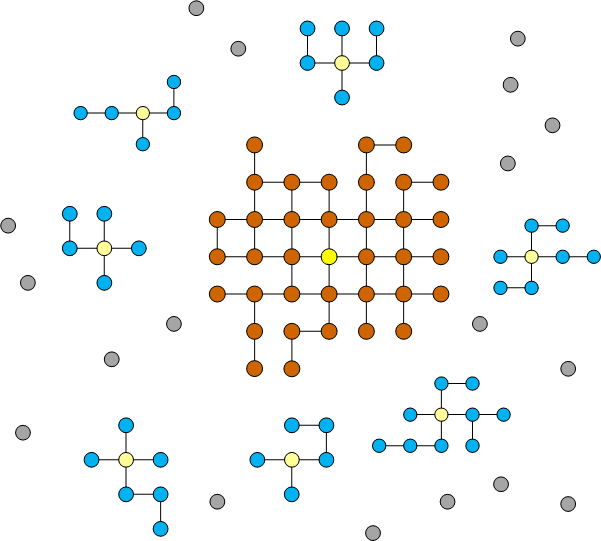
\includegraphics[scale=0.3]{slika-primer.png}
% \caption{Vsako sliko opremi s podnapisom, ki pove, kaj slika prikazuje.}
% \label{slika1}
% \end{center}
% \end{figure}
%
% V to poglavje lahko tudi vključiš kakšen metodološko zanimiv del
% kode. Primer vključitve kode oziroma implementirane funkcije v
% programskem jeziku Python je:
%
% \begin{lstlisting}
% def fib(n):
%     if n == 0:
%         return 0
%     elif n == 1:
%         return 1
%     else:
%         return fib(n-1) + fib(n-2)
% \end{lstlisting}
%
% Izris te kode je lahko sicer tudi lepši, poskušaš lahko najti še
% primernejši način vključevanja kode v Pythonu oziroma v tvojem izbranem
% programskem jeziku v okolje \LaTeX{}.

\subsection{Regresija}
Pred gradnjo in vrednotenjem modelov je bilo potrebno podatke spraviti v
ustrezno obliko.

Podatke sem prebral in jih pretvoril v matriko filmov in uporabnikov.

\begin{lstlisting}
dfRatings = pd.read_csv('../data/ratings.csv')

# transform df
df = dfRatings.pivot(index='movieId', columns='userId', values='rating')
\end{lstlisting}

Iz podatkov sem nato odstranil vse filme z manj kot 100 ocenami, iz dobljene
matrike sem nato odstranil še vse uporabnike z manj kot 100 ocenami.

\begin{lstlisting}
# drop movies with less than 100 ratings
df.dropna(axis=0, how='any', thresh=100, subset=None, inplace=True)

# drop users with less than 100 ratings
df.dropna(axis=1, how='any', thresh=100, subset=None, inplace=True)
\end{lstlisting}

Pred začetkom granjem modelov je bilo potrebno poskrbeti še za neznane vrednosti.
Le te sem zamenjal z oceno 0.

\begin{lstlisting}
# replace null values with 0
df = df.fillna(0)
\end{lstlisting}

Za regresijo sem izbral tri modele Linear regression, Lasso in Bayesian Ridge.

Učenja modelov sem se lotil tako, da sem za vsakega uporabnika iz matrike trikrat
naključno izbral primere za učno in testno množico, naučil model s podatki iz
učne množice in ga ovrednotil s pomočjo testne množice. Uporabnika za katerega
sem gradil model, sem uporabil le kot ciljno spremenljivko, zato sem njegove
ocene iz učne in testne množice odstranil.

\begin{lstlisting}
for user in df.columns:
    for x in range(3):
        # split df into training and test sets
        trainDf = df.sample(frac=.75)
        testDf = df[~df.index.isin(trainDf.index)]

        # get ratings of current user
        trainUserDf = trainDf.loc[:, user].copy()
        testUserDf = testDf.loc[:, user].copy()

        # drop current user from training and test sets
        trainDf = trainDf.drop(user, 1)
        testDf = testDf.drop(user, 1)

        ### learn and evaluate models ###
\end{lstlisting}

Za ovrednotenje modelov sem izbral mero Mean Absolute Error, ker se mi je ta
mera zdela najlažja za razumevanje kako dobro oz. slabo napoveduje model.
Dobljena ocena MAE pove, za koliko se v povprečju zmoti model pri napovedovanju
novih vrednosti.

\begin{lstlisting}
def learnPredictScore(model, trainX, trainY, testX, testY):
    model.fit(trainX, trainY)

    # predict ratings for current user
    prediction = model.predict(testX)

    # MAE
    return mean_absolute_error(prediction, testY)
\end{lstlisting}


\subsection{Klasifikacija}
Priprava podatkov za klasifikacijo je potekala na enak način kot pri regresiji. Vrednosti v matriki filmov in uporabnikov sem pretvoril v dva razreda, 0 če je bila ocena manjša ali enaka 3, sicer 1.

\begin{lstlisting}
df = df.applymap(lambda x: 1 if x > 3 else 0)
\end{lstlisting}

Za vsakega uporabnika iz matrike sem trikrat naključno izbral primerke za učno in testno množico, naučil modele ter jih ovrednotil s pomočjo klasifikacijske točnosti in ocene F1.

\subsection{Bonus}
V matriko filmov in uporabnikov sem dodal novega uporabnika z mojimi ocenami filmov. Ocenil sem 16 filmov, ostali filmi v matriki so bili tako kot pri ostalih uporabnikih ocenjeni z oceno 0.

\begin{lstlisting}
myRatings = [4, 5, 0, 0, 0, 0, 0, 0 ,0, 4, 0, 0, 0, 0,
             3, 0, 0, 0, 0, 1, 0, 5, 0, 0, 0, 0, 0, 0,
             4, 0, 5, 0, 0, 4, 4, 2, 0, 4, 5, 5, 5, 0, 5]
myRLen = len(myRatings)

for x in range(len(df)-myRLen):
    myRatings.append(0)

user = 9999

df2 = pd.DataFrame({user:myRatings}, index = df.index)

df = pd.concat([df,df2], axis=1)
\end{lstlisting}

Za novega uporabnika sem zgradil regresijski model s pomočjo metode Lasso in napovedal ocene za preostale filme.

\section{Rezultati}

% V tem poglavju podaš rezultate s kratkim (enoodstavčnim)
% komentarjem. Rezultate lahko prikažeš tudi v tabeli (primer je
% tabela~\ref{tab1}).

% Odstavke pri pisanju poročila v LaTeX-u ločiš tako, da pred novim
% odstavkom pustiš prazno vrstico. Tudi, če pišeš poročilo v kakšnem
% drugem urejevalniku, morajo odstavki biti vidno ločeni. To narediš z
% zamikanjem ali pa z dodatnim presledkom.

% \begin{table}[htbp]
% \caption{Atributi in njihove zaloge vrednosti.}
% \label{tab1}
% \begin{center}
% \begin{tabular}{llp{3cm}}
% \hline
% ime spremenljivke & definicijsko območje & opis \\
% \hline
% cena & [0, 500] & cena izdelka v EUR\\
% teža & [1, 1000] & teža izdelka v dag \\
% kakovost & [slaba|srednja|dobra] & kakovost izdelka \\
% \hline
% \end{tabular}
% \end{center}
% \end{table}

% Podajanje rezultati naj bo primerno strukturirano. Če ima naloga več
% podnalog, uporabi podpoglavja. Če bi želel poročati o rezultatih
% izčrpno in pri tem uporabiti vrsto tabel ali grafov, razmisli o
% varianti, kjer v tem poglavju prikažeš in komentiraš samo glavne
% rezultate, kakšne manj zanimive detajle pa vključite v prilogo (glej
% prilogi~\ref{app-res} in~\ref{app-code}).
\subsection{Regresija}
V tabeli~\ref{tab1} so prikazani rezultati vseh treh modelov. Za najslabšega se je
izkazal model zgrajen z linearno regresijo, medtem ko sta Lasso in Bayesian Ridge
vračala skoraj identične rezultate.


\begin{table}[htbp]
\caption{Rezultati modelov za regresijo}
\label{tab1}
\begin{center}
\begin{tabular}{lp{4cm}}
\hline
model & mean absolute error \\
\hline
Linear regression & 1.3557 \\
Lasso & 1.2347 \\
BayesianRidge & 1.2379 \\
\hline
\end{tabular}
\end{center}
\end{table}

\subsection{Klasifikacija}

Z modelom SVM sem uspel napoved v primerjavi z večinskim klasifikatorjem izboljšati
za približno 14\%.

\begin{table}[htbp]
\caption{Rezultati modela SVM za klasifikacijo}
\label{tab2}
\begin{center}
\begin{tabular}{lp{4cm}}
\hline
mera & rezultat \\
\hline
večinski klasifikator & 0.5467 \\
klasifikacijska točnost & 0.6847 \\
F1 & 0.6471 \\
\hline
\end{tabular}
\end{center}
\end{table}

Klasifikacijski problem je lažji od regresijskega, saj je pri klasifikaciji nabor vrednosti
precej manjši kot pri regresiji, kjer napovedujemo vrednost v zveznem prostoru.

\subsection{Bonus}
Ocenil sem 16 od 151 filmov, kar se je izkazalo za premalo, da bi lahko model vrnil uporabne
napovedi. Večina ocen se je gibala med 1 in 2. Algoritem je pravilno višje ocenil animirane filme,
ni pa uspel razpoznati povezave med nadaljevanji filmov. Napoved se pri majhnem številu ocenjenih
filmov ni izkazala za uporabno.

\section{Izjava o izdelavi domače naloge}
Domačo nalogo in pripadajoče programe sem izdelal sam.

\appendix
\appendixpage
\section{\label{app-res}Podrobni rezultati poskusov}

% Če je rezultatov v smislu tabel ali pa grafov v nalogi mnogo,
% predstavi v osnovnem besedilu samo glavne, podroben prikaz
% rezultatov pa lahko predstaviš v prilogi. V glavnem besedilu ne
% pozabi navesti, da so podrobni rezultati podani v prilogi.



\section{\label{app-code}Programska koda}

% Za domače naloge bo tipično potrebno kaj sprogramirati. Celotno kodo oddaj
% zapakirano skupaj s poročilom v datoteki zip. V kolikor je določen izsek kode
% nujen za boljše razumevanje poročila, ga vključi v prilogo poročila.

% Čisto
% za okus sem tu postavil nekaj kode, ki uporablja Orange
% (\url{http://www.biolab.si/orange}) in razvrščanje v skupine.


% \begin{lstlisting}
% import random
% import Orange

% data_names = ["iris", "housing", "vehicle"]
% data_sets = [Orange.data.Table(name) for name in data_names]

% print "%10s %3s %3s %3s" % ("", "Rnd", "Div", "HC")
% for data, name in zip(data_sets, data_names):
%     random.seed(42)
%     km_random = Orange.clustering.kmeans.Clustering(data, centroids = 3)
%     km_diversity = Orange.clustering.kmeans.Clustering(data, centroids = 3,
%         initialization=Orange.clustering.kmeans.init_diversity)
%     km_hc = Orange.clustering.kmeans.Clustering(data, centroids = 3,
%         initialization=Orange.clustering.kmeans.init_hclustering(n=100))
%     print "%10s %3d %3d %3d" % (name, km_random.iteration, \
%     km_diversity.iteration, km_hc.iteration)
% \end{lstlisting}

\end{document}
